\chapter{Implementing a SyntaxRewriter}
\label{sec:syntaxrewriter}

A \textbf{SyntaxRewriter} is very similar to the SyntaxWalker we saw in chapter \ref{sec:syntaxwalker} and provides us with a clean \gls{api} which we can use to, as the name gave away, rewrite certain parts of the \gls{syntaxtree}. Here, too, we are working on the syntactic level so we can't make use of the 'smarter' \gls{semanticmodel} and accompanying symbols. However, the scenario we will look at suffices perfectly with just syntactic knowledge so there's no problem here.

A common dispute\footnote{\url{http://stackoverflow.com/q/4540146/1864167}} between C\# programmers is whether to use an underscore as a prefix for private fields. This makes a great scenario for us to test a SyntaxRewriter: we will change all \texttt{private} fields to use an underscore as prefix. Again we will ignore the scenario where no access modifier is defined and just pretend that we don't handle those to keep focus on the rewriter itself.

Just like the SyntaxWalker, we have to start by parsing our source code as a \gls{syntaxtree}. Once we have that, we do the same thing as we did before: retrieve the root node and start traversing your tree from there. After all defined transformations have been applied, we will format the newly generated tree and display it (listing \ref{lst:syntaxrewriter-getting-started}). Important to note: the tree we pass in and get back are \textit{not} the same: everything is \gls{immutable} in Roslyn (more on that in section \ref{sec:syntax-tree}).

\clearpage

\lstset{style=csharp, caption={Getting started with a SyntaxRewriter}}
\begin{minipage}{\linewidth}
\begin{lstlisting}[label={lst:syntaxrewriter-getting-started}]
const string source = @"
	public class MyOuterClass
	{
	    private int _myField;
	    private string anotherField;
	    private double x, _y;
	    
	
	    private class MyInnerClass
	    {
	        private int _innerField;
	        public int anotherInnerField;
	    }
	}
";
var tree = CSharpSyntaxTree.ParseText(source);
var rewriter = new MyRewriter().Visit(tree.GetRoot());
var formattedTree = Formatter.Format(rewriter, Formatter.Annotation, new AdhocWorkspace());
Console.WriteLine(formattedTree.ToFullString());
\end{lstlisting}
\end{minipage}

When you think of a field declaration it (typically) consists of several aspects. Take the following line for example: 

\lstset{style=csharp, caption={Example of a FieldDeclaration}}
\begin{lstlisting}[label={lst:syntaxrewriter-example-fielddeclaration}]
private int x, y = 10;
\end{lstlisting}

This in its entirety is a \texttt{FieldDeclarationSyntax}. Looking at the next level, we can find a \texttt{VariableDeclarationSyntax}:

\lstset{style=csharp, caption={Extracted VariableDeclaration}}
\begin{lstlisting}[label={lst:syntaxrewriter-example-variabledeclaration}]
int x, y = 10
\end{lstlisting}

One level further, we can finally find the \texttt{VariableDeclaratorSyntax} (listing \ref{lst:syntaxrewriter-example-variabledeclarators}). It's this declarator that will contain the information we're looking for: the identifier. This example also immediately shows a tricky aspect to our rewriter: multiple variables can be defined in one field declaration so this is something we have to support.

\lstset{style=csharp, caption={Extracted VariableDeclarators}}
\begin{lstlisting}[label={lst:syntaxrewriter-example-variabledeclarators}]
x 			// First declarator
y = 10 	// Second declarator
\end{lstlisting}

The importance of realizing everything is \gls{immutable} really shows itself in listing \ref{lst:syntaxrewriter-implementing-syntaxrewriter}. Here we override the \texttt{VisitFieldDeclaration} method which is triggered every time the rewriter comes across a field. We can also see that the method returns a \texttt{SyntaxNode} which will be the \texttt{FieldDeclarationSyntax} we construct with the new identifier.

\noindent When we look at the implementation of this method we can distinguish a few steps:

\begin{itemize}
\item Create a container to store declarators
\item Get all identifiers from our field declaration
\item Create a new identifier for each \texttt{private} identifier that does not start with an underscore
\item Create a new declarator for each newly created identifier
\item Create a new declaration based on the (potentially) new declarators
\item Create a new field based on this new declaration and add the \texttt{Formatter} annotation to it so we can properly format the changed nodes afterwards
\end{itemize}

Immediately it's clear that we will have to create a lot of new objects to represent our changed syntax nodes. This is a result of the public Roslyn \gls{api} being \gls{immutable} but luckily there are a lot of useful factory methods available in \texttt{SyntaxFactory} to create those elements for us. This also represents the key consideration when manipulating a \gls{syntaxtree}: when a node is changed, every ancestor node will also be changed up until the highest level which can be a simple root node or possibly a \texttt{Document} or \texttt{Solution}. In our rewriter we should only replace until the level that was visited: a field declaration. Internally, the rewriter will then do the additional replacing by itself.

\clearpage

\lstset{style=csharp, caption={Implementing the SyntaxRewriter}}
\begin{lstlisting}[label={lst:syntaxrewriter-implementing-syntaxrewriter}]
public override SyntaxNode VisitFieldDeclaration(FieldDeclarationSyntax node)
{
	var newDeclarators = 
		new List<VariableDeclaratorSyntax>();

	foreach (var declarator in node.Declaration.Variables)
	{
		var currentIdentifier = declarator.Identifier;
		if (!currentIdentifier.ValueText.StartsWith("_") && 
				node.Modifiers.Any(
					x => x.Kind() == SyntaxKind.PrivateKeyword))
		{
			var newIdentifier = 
				SyntaxFactory.Identifier(
					currentIdentifier.LeadingTrivia, 
					"_" + currentIdentifier.ValueText, 
					currentIdentifier.TrailingTrivia);
					
			var newDeclarator = 
				declarator.WithIdentifier(newIdentifier);
				
			newDeclarators.Add(newDeclarator);
		}
		else
		{
			newDeclarators.Add(declarator);
		}
	}
	
	var newDeclaration = 
		SyntaxFactory.VariableDeclaration(
			node.Declaration.Type, 
			SyntaxFactory.SeparatedList(newDeclarators));
			
	return 
		SyntaxFactory.FieldDeclaration(
			node.AttributeLists, 
			node.Modifiers, 
			newDeclaration)
		.WithAdditionalAnnotations(Formatter.Annotation);
}
\end{lstlisting}

\begin{minipage}{\linewidth}
\noindent The resulting source code after our transformation can be seen in figure \ref{syntaxrewriter-results}.

There are a lot of interesting use cases this opens up. Think for example about a build system where every user specifies their preferred naming conventions and when checking in and checking out source code, it will automatically transform it to the requested representation. This would eliminate the eternal discussion about coding styles entirely! Large refactorings are made easier by this as well: if you change from one convention or idiom to another, creating a SyntaxRewriter might take away a lot of the pain that typically comes with something like that.

\begin{figure}[H]
\centering
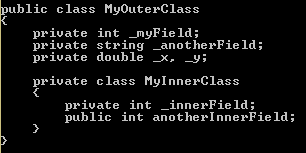
\includegraphics[scale=1]{syntaxrewriter-results}
\caption[Renaming fields with a SyntaxRewriter]{Renaming fields with a SyntaxRewriter}
\label{syntaxrewriter-results}
\end{figure}
\end{minipage}